\documentclass{article}

\usepackage{amsmath,amssymb}
\usepackage{tikz}
\usepackage{pgfplots}
\usepackage{xcolor}
\usepackage[left=2.1cm,right=3.1cm,bottom=3cm,footskip=0.75cm,headsep=0.5cm]{geometry}
\usepackage{enumerate}
\usepackage{enumitem}
\usepackage{marvosym}
\usepackage{tabularx}
\usepackage{parskip}
\usepackage{longtable}

\usepackage{listings}
\definecolor{lightlightgray}{rgb}{0.95,0.95,0.95}
\definecolor{lila}{rgb}{0.8,0,0.8}
\definecolor{mygray}{rgb}{0.5,0.5,0.5}
\definecolor{mygreen}{rgb}{0,0.8,0.26}
\lstdefinestyle{R} {language=R}
\lstdefinestyle{Python} {language=Python}
\lstset{language=SQL,
	basicstyle=\ttfamily,
	keywordstyle=\color{lila},
	commentstyle=\color{lightgray},
	stringstyle=\color{mygreen}\ttfamily,
	backgroundcolor=\color{white},
	showstringspaces=false,
	numbers=left,
	numbersep=10pt,
	numberstyle=\color{mygray}\ttfamily,
	identifierstyle=\color{blue},
	xleftmargin=.1\textwidth, 
	%xrightmargin=.1\textwidth,
	escapechar=§,
	%literate={\t}{{\ }}1
	breaklines=true,
	postbreak=\mbox{\space},
	morekeywords={with, data, refresh, materialized, explain, rank, over, partition, uuid, extension, replace, function, returns, language}
}

\usepackage[colorlinks = true, linkcolor = blue, urlcolor  = blue, citecolor = blue, anchorcolor = blue]{hyperref}
\usepackage[utf8]{inputenc}

\renewcommand*{\arraystretch}{1.4}

\newcolumntype{L}[1]{>{\raggedright\arraybackslash}p{#1}}
\newcolumntype{R}[1]{>{\raggedleft\arraybackslash}p{#1}}
\newcolumntype{C}[1]{>{\centering\let\newline\\\arraybackslash\hspace{0pt}}m{#1}}

\newcommand{\E}{\mathbb{E}}
\DeclareMathOperator{\rk}{rk}
\DeclareMathOperator{\Var}{Var}
\DeclareMathOperator{\Cov}{Cov}

\title{\textbf{Scalable Data Engineering, Lösungsvorschlag Test Exam WS 2022/23}}
\author{\textsc{Henry Haustein}}
\date{}

\begin{document}
	\maketitle
	
	\section*{Question 1: Multidimensional Modelling}
	\begin{enumerate}[label=(\alph*)]
		\item This is the same as exercise 1, task 4. I decided to don't introduce a \texttt{movie ID} but instead make \texttt{movie title} and \texttt{prod-year} a primary key. Software like KODI (\url{https://kodi.tv/}) and Plex (\url{https://www.plex.tv/de/}) rely on this when they index your local collection of movies.
		\begin{center}
			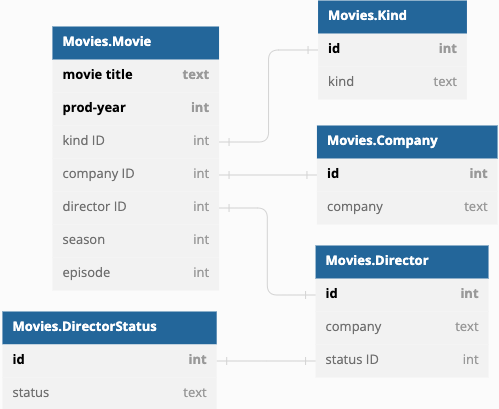
\includegraphics[scale=0.5]{Test Exam Q1}
		\end{center}
		\item It's a Snowflake schema since the schema is fully normalised.
	\end{enumerate}

	\section*{Question 2: Reporting functions}
	SQL, not tested (I don't have a pgAdmin at hand right now)
	\begin{lstlisting}[tabsize=2]
SELECT P_NAME, SUM(L_QUANTITY) AS qty
FROM PART, LINEITEM
WHERE P_PARTKEY = L_PARTKEY
GROUP BY L_PARTKEY
ORDER BY 2 DESC
	\end{lstlisting}

	\section*{Question 3: Schema Matching}
	\begin{enumerate}[label=(\alph*)]
		\item Bigram representations:
		\begin{itemize}
			\item firstname: \_f, fi, ir, rs, st, tn, na, am, me, e\_
			\item lastname: \_l, la, as, st, tn, na, am, me, e\_
			\item street: \_s, st, tr, re, ee, et, t\_
			\item name: \_n, na, am, me, e\_
			\item adress: \_a, ad, dr, re, es, ss, s\_
			\item forename: \_f, fo, or, re, en, na, am, me, e\_
		\end{itemize}
		\item Bigramm scores
		\begin{center}
			\begin{tabular}{l|l|l|l}
				& \textbf{firstname} & \textbf{lastname} & \textbf{street} \\
				\hline
				\textbf{name} & $\frac{2\cdot 4}{10+5}=0.533$ & $\frac{2\cdot 2\cdot 4}{9+5}=0.571$ & $\frac{2\cdot 0}{7+5}=0$ \\
				\hline
				\textbf{address} & $\frac{2\cdot 0}{10+8}=0$ & $\frac{2\cdot 0}{9+8}=0$ & $\frac{2\cdot 1}{7+8}=0.133$ \\
				\hline
				\textbf{forename} & $\frac{2\cdot 5}{10+9}=0.526$ & $\frac{2\cdot 4}{9+9}=0.444$ & $\frac{2\cdot 1}{7+9}=0.125$
			\end{tabular}
		\end{center}
		Stable Marriage Algorithm:
		\begin{itemize}
			\item firstname proposes to name, agrees: (firstname, name)
			\item lastname proposes to name, agrees + leaves: (lastname, name)
			\item firstname proposes to forename, agrees: (lastname, name), (firstname, forename)
			\item street proposes to adress, agrees: (lastname, name), (firstname, forename), (street, adress)
		\end{itemize}
	\end{enumerate}

	\section*{Question 4: Time Series Data}
	Trend extraction via moving average with window size 7. Then $trend(1)$, $trend(2)$ and $trend(3)$ all NULL
	\begin{align}
		trend(4) &= avg(8,10,11,12,16,17,20) = 13.429 \notag \\
		trend(5) &= avg(10,11,12,16,17,20, 24) = 15.714 \notag \\
		trend(6) &= avg(11,12,16,17,20, 24, 23) = 17.571 \notag
	\end{align}
	$trend(7)$, $trend(8)$ and $trend(9)$ are then NULL again.
	
	\section*{Question 5: Word Embedding Training}
	In the input layer we input the vector representation (dimensionality is 10) of every word which is in the sentence (6 words). So we need 60 neutrons.
	
	The hidden layer size is 10 as stated in the task.
	
	In the output layer we want a probability for every words, so we need there 500 neurons.
	
\end{document}